\documentclass[../main/main.tex]{subfiles}

% Put everything that shall appear in the results
% inside this document environment.
\begin{document}
In this chapter we present several plots showing the results of our experiment evaluations, starting with general averaged evaluations before presenting individual task performance and bier scores.
\subsection{Demographical Data}
Our questionare shown in \ref{appendix:questionaire} has been evaluated on 14 subjects. Their average age was 31.5 years within a range of our youngest 22 year old subject and our oldest subject of 62 years. The group consisted of 6 females and 8 males, all with german nationality and german as their mother language. Their professions included one computer scientist, one scientific coworker, one social worker, one curative educator, one insurance agent and nine students. The subjects of the later included \textit{Psychology in IT} in 5 times and \textit{Computer Science} in two times. One student's subject was \textit{Social Works}, one was studying \textit{Psychology} and one student came from \textit{Cognitive Science}.
\subsection{Averaged Task Performance and Brier Score}
The average task performence of our subjects is shown in \ref{fig:avg_scores}, with an absulate mean of [TODO: X], averaged across subjects and across tasks. 
\begin{figure}[h]
	\centering
	\captionsetup{justification=centering}
	\label{fig:avg_scores}
	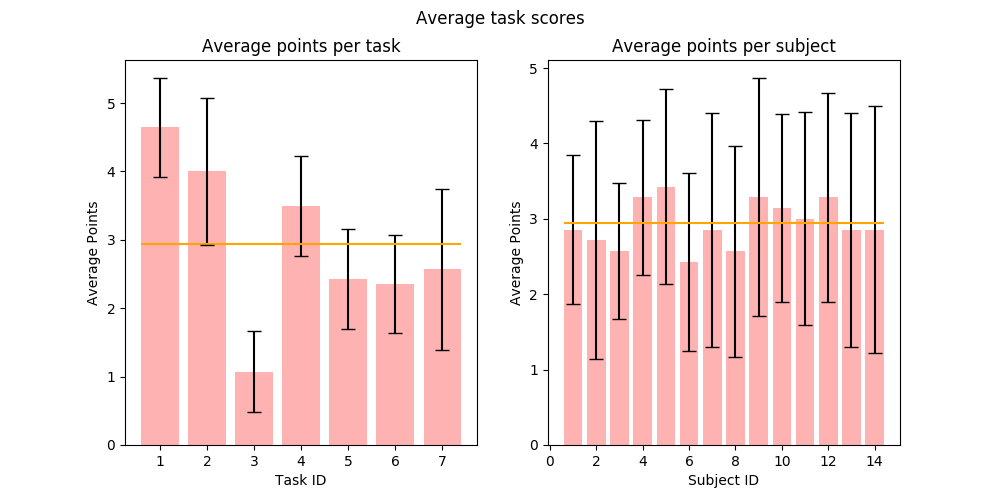
\includegraphics[width=\textwidth]{../assets/average_task_scores.png}
	\caption{Means and standard deviations of the achieved task scores, averaged over subjects in the left and over tasks in the right plot. The orange line displays the overall mean of [TODO], averaged over both variables.]}
\end{figure}
The subjects abilities to judge about their own performance, encode by the average brier score, is displayed in figure \ref{fig:avg_brier} with an overall average of 0.14. 
\begin{figure}[h]
	\centering
	\captionsetup{justification=centering}
	\label{fig:avg_brier}
	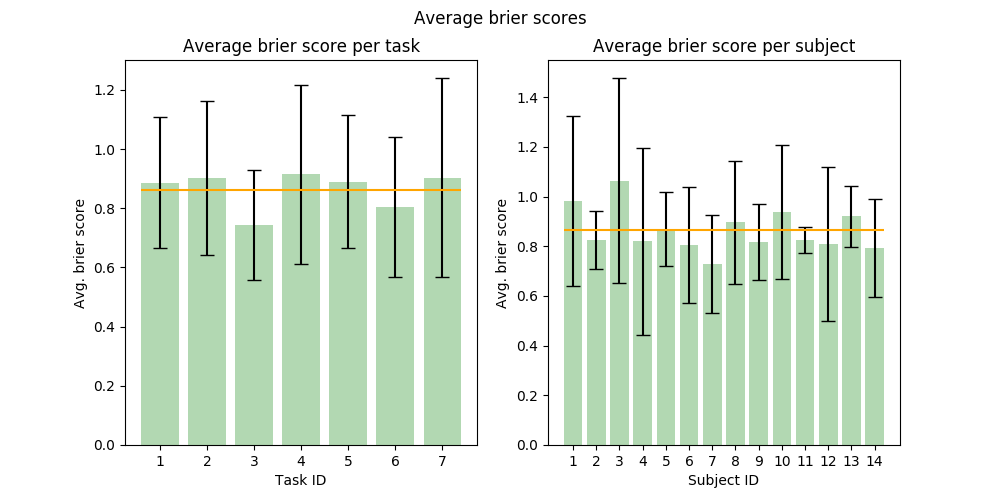
\includegraphics[width=\textwidth]{../assets/average_brier_scores.png}
	\caption{Means and standard deviations of the calculated brier scores, averaged over subjects in the left and over tasks in the right plot. The orange line displays the overall mean of 0.14, averaged over both variables.]} 
\end{figure}
Please note that we excluded the 8th task from our questionaire in \ref{appendix:questionaire}. For interpretation of these values, please refer to our discussion section \ref{sec:discussion}.
\subsection{Individual Evaluations}
\subsection{Overal Confidence}
\subsection{Task performance vs Brier Score}
\subsection{Calibrations}
\end{document}